\documentclass[a4paper, 10pt]{article}
\usepackage{helvet}
\renewcommand{\familydefault}{\sfdefault}
\usepackage{pgf}
\usepackage{eurosym}
\usepackage{graphicx}
\usepackage{wasysym}
\usepackage{hyperref}
\usepackage{listings}
\usepackage{pxfonts}
\usepackage{verbatim}
\usepackage{color}
\usepackage{xcolor}
\usepackage{wrapfig}
\usepackage{enumitem}
\usepackage{booktabs}
\usepackage{gensymb}
\usepackage{tabularx}
\usepackage{currfile}

\hypersetup{
    bookmarks=true,         % show bookmarks bar?
    unicode=true,          % non-Latin characters in Acrobat’s bookmarks
    pdftoolbar=true,        % show Acrobat’s toolbar?
    pdfmenubar=true,        % show Acrobat’s menu?
    pdffitwindow=true,     % window fit to page when opened
    pdftitle={Assessments},    % title
    pdfauthor={Paul Vesey},     % author
    pdfsubject={Building Information Modelling },   % subject of the document
    pdfcreator={},   % creator of the document
    pdfproducer={xelatex}, % producer of the document
    pdfkeywords={'Graphics' }, % list of keywords
    pdfnewwindow=true,      % links in new PDF window
    colorlinks=true,       % false: boxed links; true: colored links
    linkcolor=violet,          % color of internal links (change box color with linkbordercolor)
    citecolor=magenta,        % color of links to bibliography
    filecolor=red,      % color of file links
    urlcolor=blue           % color of external links
}

\setlength\parindent{0pt}
\begin{document}

\lstset{language=HTML,
				basicstyle=\small,
				breaklines=true,
        numbers=left,
        numberstyle=\tiny,
        showstringspaces=false,
        aboveskip=-20pt,
        frame=leftline
        }
				
\begin{figure}
	\centering
	
\includegraphics[width=0.5\linewidth]{./Assignments/img/LITlogo}
\end{figure}


\begin{tabularx}{\textwidth}{ |l|X| }
	\hline
	\textbf{Subject:} & Revit MEP\\
	\textbf{Course:} & Building Information Modelling with Revit MEP\\
	\textbf{Session:} & Autumn 2021\\
	\textbf{Lecturer:} & Paul Vesey \footnotesize{BEng, MIE, HDip}\\
	\textbf{Filename:} & \currfilebase\\
	\hline
\end{tabularx}



\vspace{0.25cm}	
	
\begin{flushleft}
\Large\textbf{Assignment 1 (33\%) - Detached 2 Storey Residence with Dormer Window}\\
\end{flushleft}

\begin{tabular}{|l|l|}
	\hline 
	Issue Date & As per Moodle \\ 
	\hline 
	Submission Date & As per Moodle \\ 
	\hline 
\end{tabular} 
\\

\large\textbf{Assignment Outline}\\

You are required to model a two storey house incorporating a dormer window and to digitally submit you project file (.rvt) showing your model on one A4 sheet and three A1 sheets.

\large\textbf{Your Submission should contain the following information}\\


\textbf{Sheet 1:} Sheet Size - A4, Sheet No - A101, Sheet Name - Cover Sheet
\begin{itemize}
	\item Three Dimensional (Aerial View) of the model (scaled to suit the sheet size) Shaded
	\item A list of the drawings in the design pack
\end{itemize}


\textbf{Sheet 2:} Sheet Size - A1, Sheet No - A102, Sheet Name - Floor Plans
\begin{itemize}
	\item Ground and First Floor Plans @ 1:50 with dimensions, Room Titles ans some fixed furniture
	\item Two internal camera views, (scaled to suit the sheet size) rendered using the Autodesk 360 cloud rendering service.  \textit{One of the fireplace and one of the kitchen units} 
\end{itemize}


\textbf{Sheet 3:} Sheet Size - A1, Sheet No - A103, Sheet Name - Elevations
\begin{itemize}
	\item South Elevation @ 1:50
	\item North, East and West Elevations @ 1:100
\end{itemize}

\textbf{Sheet 4:} Sheet Size - A1, Sheet No - A102, Sheet Name - Sections and Details
\begin{itemize}
	\item Three sections are required
	\item Section thro' Kitchen / Sitting Room facing East (towards fireplace) @ 1:100
	\item Section thro' Kitchen / Sitting Room facing West (towards kitchen units) @ 1:100
	\item Section thro' the Hallway / Landing showing the Stairs and the Dormer @ 1:100
	\item One full height detail (Call-outs) @ 1:20, including Repeating Details showing the following:
	\begin{itemize}
		\item Foundation / External Wall / Floor Interfaces
		\item Facia / Soffit and Roof Details
		\item All necessary notes
	\end{itemize} 
\end{itemize}

Additional Sheets may be submitted if so desired.

\large\textbf{Presentation and Submission}\\
\begin{enumerate}
	\item All drawing sheets must have the LIT Built Environment logo and be clearly marked 'Educational Exercise - Not for Construction
	\item You are required to submit you project as a single Revit (.rvt) file through Moodle
	\item Drawings should show all necessary information to communicate design intent
	\item The Revit filename should be of the form \textit{Semester  + Year + Project No. + First Initial + Surname + K-Number}. An example would be \textbf{'Spring18P01PVeseyK00123456.rvt'}.  Do not use spaces in the filename
\end{enumerate}


\newpage
\begin{flushleft}
\Large\textbf{Design Specification}\\
\end{flushleft}


The total floor area of the house should be approx 150$m^2$\\

The following design may be used as a guide.  You may modify the proportions provided you maintain a protrusion at the front of the building.


\begin{itemize}
	\item Enterance Hall (2400mm wide)
	\item Universilly Accessible Bathroom / Toilet
	\item Kitchen / Dining (with fixed and loose furniture)
	\item Living Room / Sitting Room (with direct access to kitchen)
	\item Ground Floor Bedroom (Playroom / Study)
	\item Externally accessed boiler house/shed
	\item Stairs 900mm wide (Rise 171.9mm, Going 280mm)
\end{itemize}



\begin{figure}
	\centering
	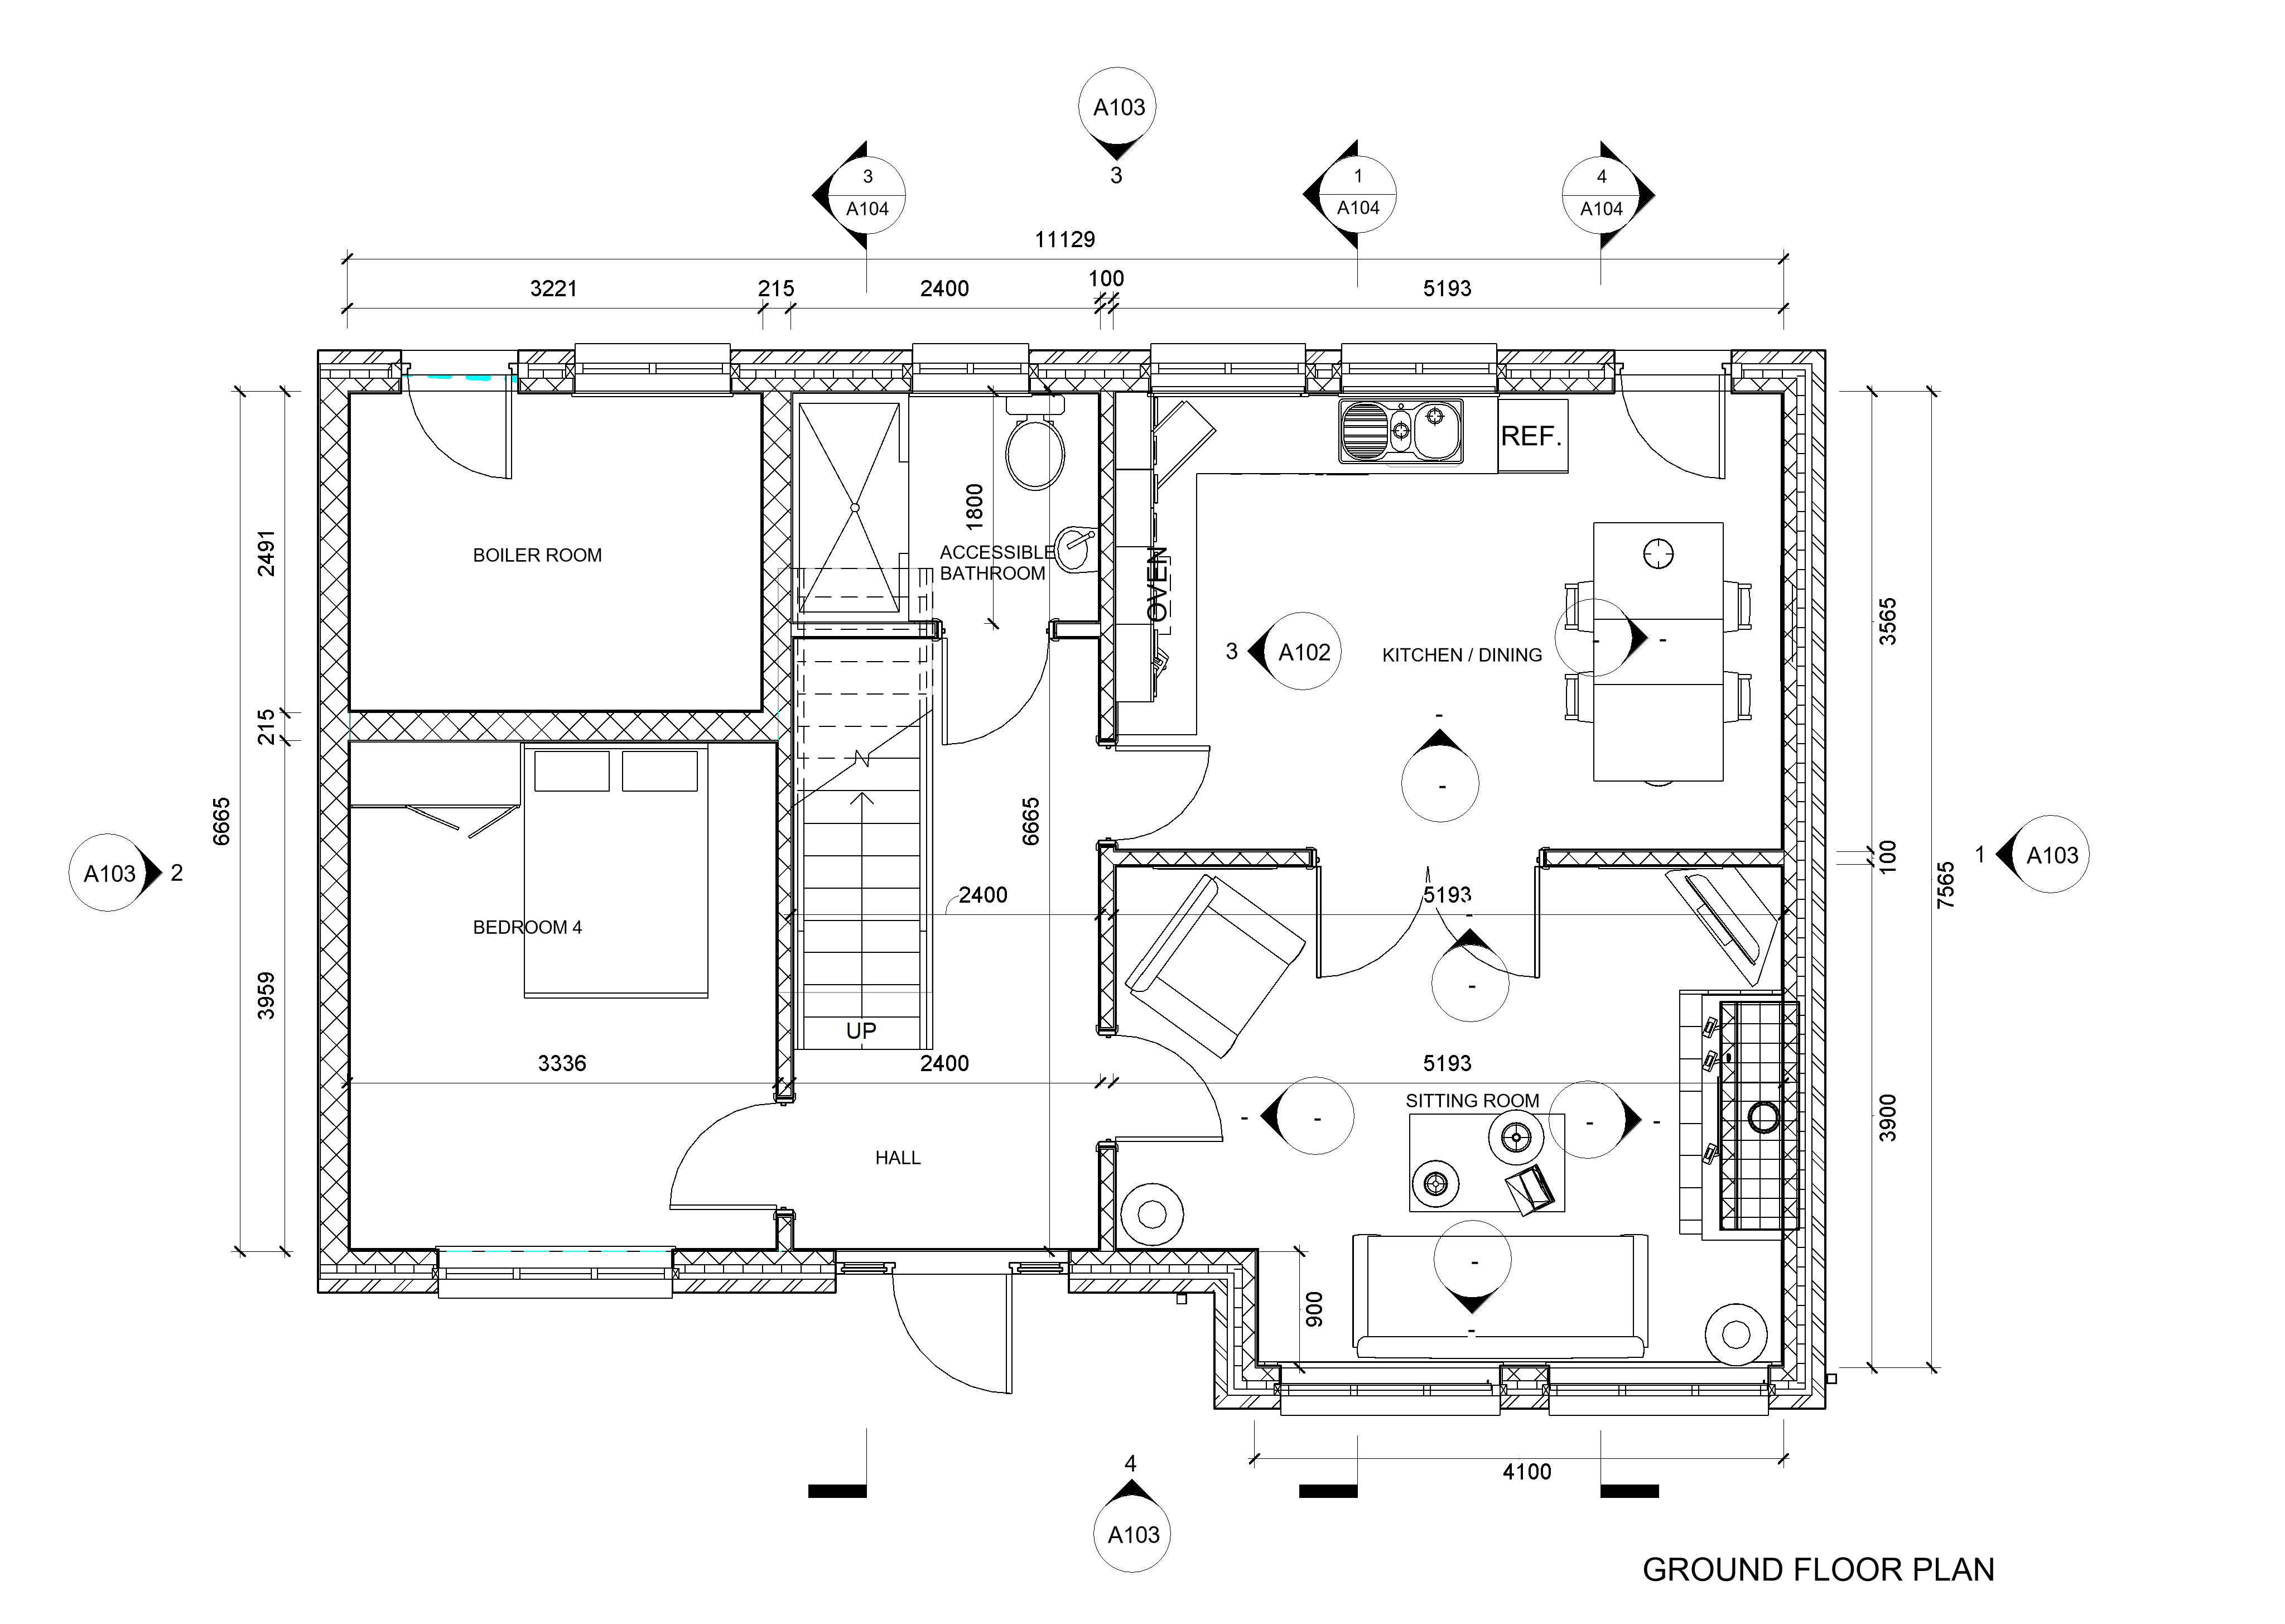
\includegraphics[width=1.0\linewidth]{img/P01GroundFloorLevel.jpg}
	\caption{Ground Floor}
	\label{fig:p01groundfloorlevel}
\end{figure}


\newpage

\begin{itemize}
	\item 3 Bedrooms with en-suite sanitary facilities
	\item Main Bathroom with Bath or Shower, WC and sink
	\item Hot Press
\end{itemize}



\begin{figure}[th]
	\centering
	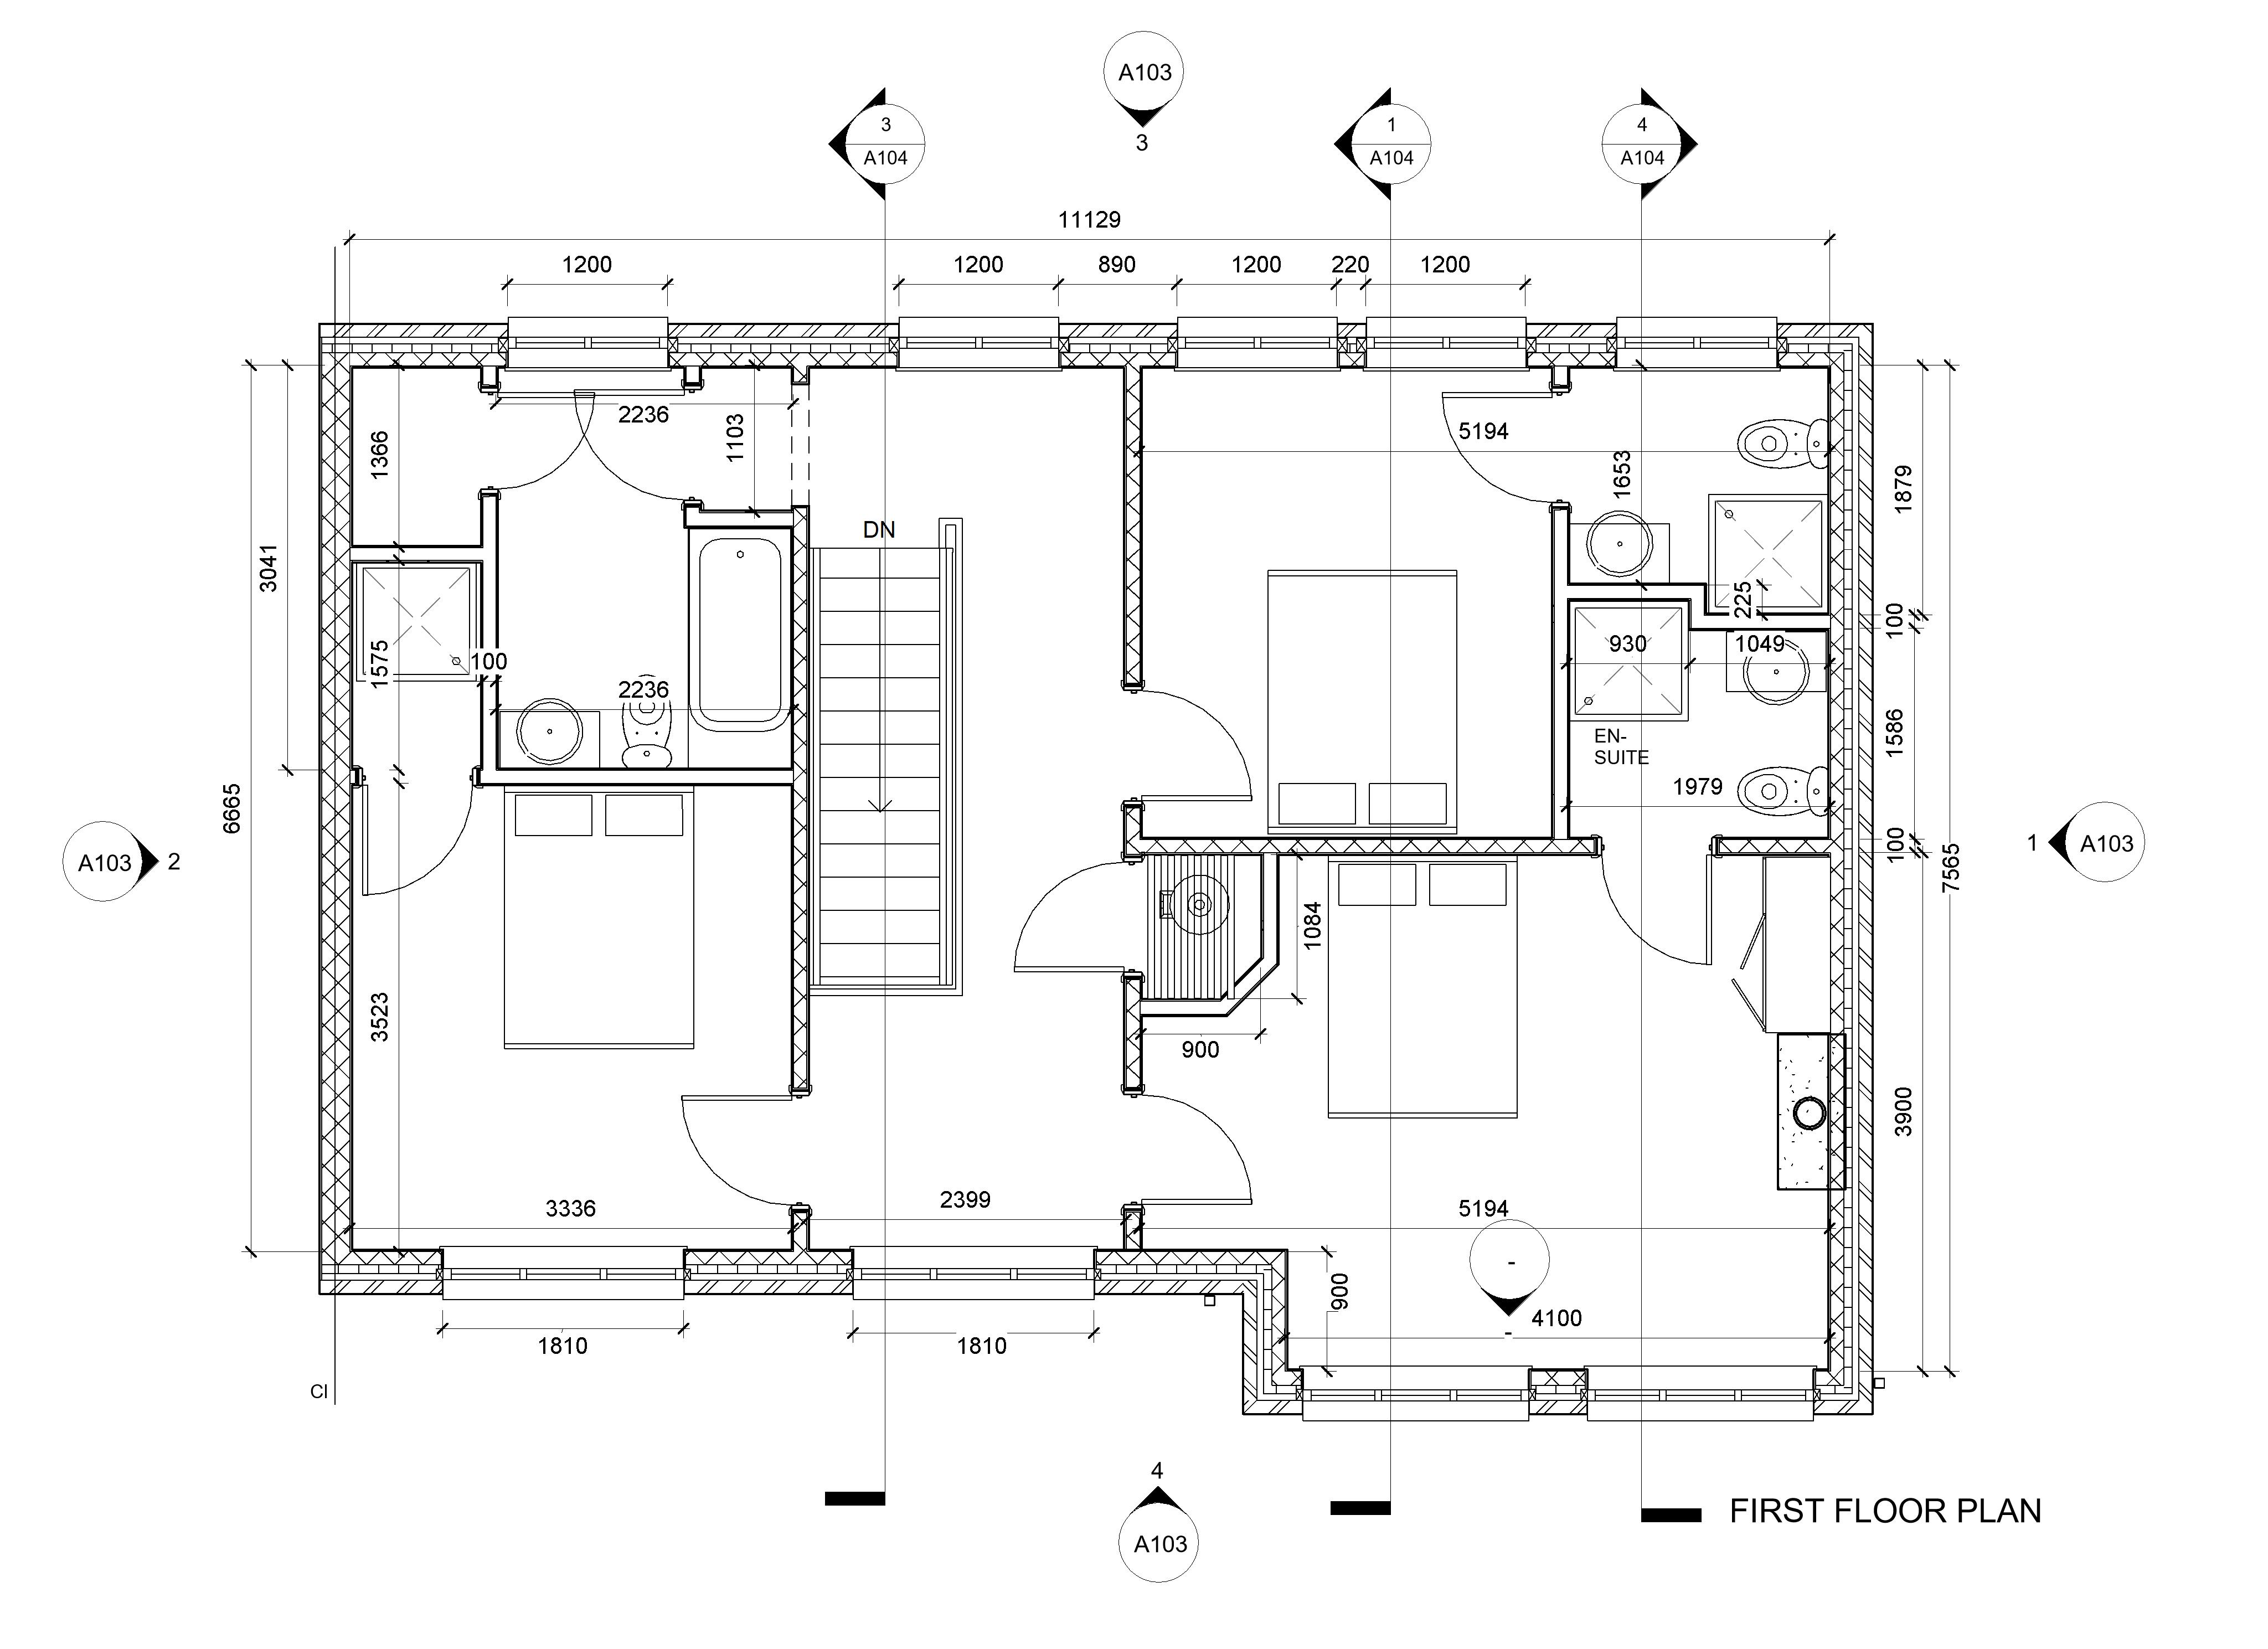
\includegraphics[width=1.0\linewidth]{img/P01FirstFloorLevel.jpg}
	\caption{First Floor Plan}
	\label{fig:p01firstfloorlevel}
\end{figure}



\begin{flushleft}
	\Large\textbf{Construction Specification}\\
\end{flushleft}

\textbf{External Wall Specification} 

External walls are to be twin leaf cavity construction and be of a 4 part Stacked Wall Type
Wall-Ext-Stacked\_317 (4-Part-Dom) with the following layers

\begin{enumerate}
	\item L1\_Wall-Ext-CAv\_102Bwk-50Air-65Ins-100DBlk-15Rnd\&P (Gen Dom)
	\begin{itemize}
		\item Layer 1 (TopLayer) 'Variable'
		\item (315mm wide insulated Cavity Walls over DPC level - Generally)
		\item Made up of 102.5mm Brick / 50mm Air-gap / 65mm Insulation / 100mm Blockwork inner leaf
		\item Internal Finish 15mm (total) Render and Plaster
	\end{itemize}
	
	\item L2\_Wall-Ext\_CAv\_15Rnd-100Blk-50Air-65Ins-100DBlk-25Ins (Plinth)
	\begin{itemize}
		\item Layer 2 (Intermediate Layer) 225mm high
		\item (315mm wide insulated Cavity Wall at Plinth level)
		\item 15mm Cement Render (Plinth) / 100mm block / 50mm Air-gap / 65mm Insulation / 100mm Block
		\item 25mm thick perimeter insulation up-stand to internal face
	\end{itemize}
	
	
	\item L3\_Wall-Ext-Cav\_100Blk-115Conc-100DBlk (Rising Wall)
	\begin{itemize}
		\item Layer 3 (Intermediate Layer) 225mm high
		\item (315mm wide un-insulated Rising Wall)
		\item 100mm Block / 115mm wide Concrete filled cavity / 100mm Block inner leaf
	\end{itemize}
	
	
	\item L4\_Wall-Solid-440\_Trench-Blk
	\begin{itemize}
		\item Layer 4 (Base Layer) 675mm high
		\item (440mm wide Solid Trench Blockwork)
	\end{itemize}
\end{enumerate}

Foundations (Footings)

\begin{itemize}
	\item 1350 wide x 450 deep strip foundation
	\item Top of Strip foundation to be 1050mm below Gr. Floor level
\end{itemize}
1350 wide x 450 deep strip foundation


\textbf{Internal Wall Specification}

Ground Floor Internal Walls
Generally, Single leaf 100mm concrete block walls 15mm render / plaster both sides
(Wall-Part\_15Rnd\&P-100Blk-15Rnd\&P)

First Floor Internal Walls 
Landing Area
Single leaf 100mm concrete block walls, 15mm render / plaster both sides
(Wall-Part\_15Rnd\&P-100Blk-15Rnd\&P)
Elsewhere
100mm timber stud partition, 15mm plaster slab / plaster both sides
(Wall-Stud-Part\_15Gwb\&P-100Stud-15Gwb\&P)


\textbf{Floor Specification}







\textbf{Windows and Doors}
\begin{itemize}
	\item Head height - 2100mm
	\item Revit Library standard door types may be used
	\item External Front Door: Decorative type (panelled door with glazed side panels)
	\item External Kitchen and Boiler house doors to have glazed panels
	\item Generally, internal single doors to be standard flush-panel or regency panelled type
	\item Kitchen to living room doors to be double leaf, glazed multi-panel style
	\item Windows generally to be double or triple sash type with opening vents
	\item Dormer window: Rectangle or circular type as desired.
\end{itemize}






\textbf{Electrical Fittings}
\begin{itemize}
	\item Kitchen and Living Room only, to be visible in Section or Camera View
	\item 2 No. Ceiling or Wall mounted light fittings per room
	\item 2 no. Twin Switched Socket power outlets per room
\end{itemize}





\textbf{Ceilings}
\begin{itemize}
	\item 3mm Skim Coat Plaster on Gypsum Wall Board
	\item Revit Library 'modified' ceiling type (Compound Ceiling Plain)
	\item Ceiling Cut-outs required for Stairs and Dormer Window.
\end{itemize}



\textbf{Roof Type}
\begin{itemize}
	\item Roof by Footprint
	\item Pitch 35\degree (also on Dormer)
	\item Main Roof overhang to be approx 300mm clear of outer leaf
	\item Dormer overhang to be approx 200mm clear of dormer walls
\end{itemize}



\textbf{Roof Construction Specification}
\begin{itemize}
	\item Revit Library roof type 'Roof\_Pitched\_38Tile-25Bat-0Felt-25Bat-100Ins-150Truss-12PBd to be modified as follows: Roof\_Pitched\_38Tile-38Bat-0Feld-150Truss. ie 38mm Roofing Tile on 38mm battens on Roof Membrane on 150mm Structure (Truss / Rafter)
\end{itemize}




\textbf{Provide the Following}
\begin{itemize}
	\item Facia Boards, Flat Soffits, Rainwater Gutters, Downpipes and all necessary information to communicate design intent.
\end{itemize}





\textbf{Site}




\textbf{How to Structure your Submission}
\\
All submission are to take the form of a single zip file.  The zip file must maintain the folder structure as generated by 3DS Max or Unity.   The images below, figure \ref{fig:3dsstructure} and figure \ref{fig:unity} give an indication of the folder structure that you should zip and submit.\\ \\

\begin{figure}[h]
	\centering
	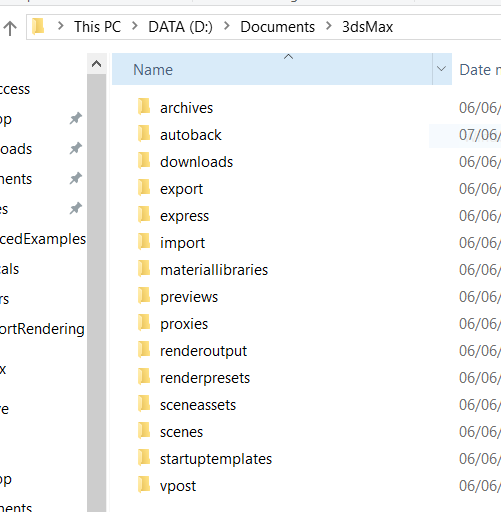
\includegraphics[width=0.5\linewidth]{img/3dsStructure.jpg}
	\caption{3D Studio Max Project Folder Structure}
	\label{fig:3dsstructure}
\end{figure}
\begin{figure}[h]
	\centering
	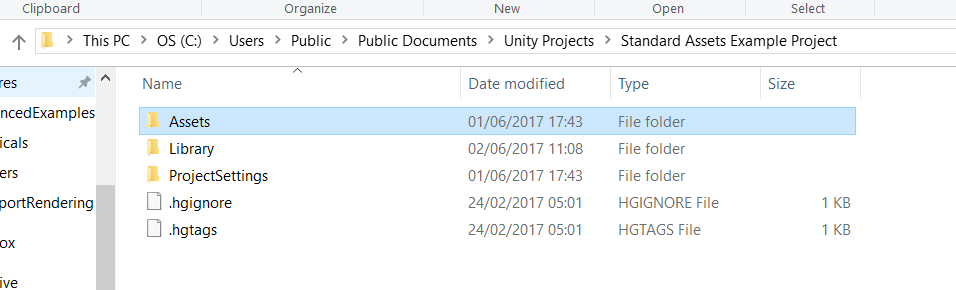
\includegraphics[width=0.9\linewidth]{img/Unity.jpg}
	\caption{Unity Game Engine File Structure}
	\label{fig:unity}
\end{figure}

All assets used during the course of the assignment are to be submitted.  All assets used and created should be placed within the appropriate folder.  To clarify, all 3ds Scene files should be placed within the 'scenes' folder; and all renders should be placed within the 'renderoutput' folder.
\\
\\
Please note that it is not appropriate to submit a single \textit{.max} file, single \textit{.jpg} file, or a single \textit{.unity} file.  

\vspace{1cm}
\textbf{Late Submission}\\
Failure to submit your assignment on or before the date and time indicated will result in a penalty of 5\% per day or part thereof.
\\
\\
Late submission penalties will not apply in cases where a valid medical certificate is provided.  In such instances an extension of time will be granted for the duration of illness stated on the medical certificate that falls after the submission date.  A copy of the medical certificate must be included with the late submission.
\\
\\
Late submission penalties may also be avoided in exceptional circumstances.  These will be dealt with on a case by case basis.  Please note that loss of pen-drives, inability to use or access the software etc. will not be considered 'exceptional circumstances'.




\end{document}